\subsection{Open/Error Message Displaying}
\label{sec:OPEN_ERROR}

Once the system has determined whether the password entered via the keypad is correct or not, an HMI (Human-Machine Interface) must be implemented. \medskip

In order to do this, we will display the result of the checking process in the 4 7-segment displays that we have already seen. 2 GALs, in combination with some special circuitry that we have fashioned ourselves will be in charge of displaying the messages: Either \textbf{\textit{Open}}, when the code entered is the correct one, or \textbf{\textit{Err}} when it is not.  

\medskip

As we have said before, each message will be processed by one GAL device due to a constraint in the number of pins. We will now go over the code of both GALs and the custom circuitry that allows us to display the messages: \medskip


\subsubsection{\textit{Open} Message}
\label{sec:OPEN_MESSAGE}

As per most of the GALs that we have used, both of them use a FSM to command the different operations. Since the codes of both are almost equal, the I/O declaration of pins will be the same. \medskip

On the one hand, as an input, we may find the signals clock (\textit{CLK}), the \textit{DONE} signal (Not the delayed version this time), the \textit{CORRECT} signal, which we thoroughly discussed in \textbf{Subsection \ref{sec:PASS_CHECK}}, the \textit{INCOMING\_PULSE} signal, which is a delayed pulse of the signal \textit{SENT\_PULSE} that again, we discussed in \textbf{Subsection \ref{sec:PASS_CHECK}} and finally, the \textit{RESET} signal, which will reset the FSM back to the original state. \medskip

On the other hand, as an output, we may find the signals \textit{NUMBER} which control the message displaying process, the \textit{DISP\_EN}, which, as the name suggests, enables the display and, finally, \textit{ENDPULSE\_SEND} which resets the whole system after a few ms, so as to allow the user to visualize the Open/Error message for a brief amount of time (See \textbf{Subsection \ref{sec:DELAYED_PULSE}} for more on this). Otherwise, the whole Opening/Error sequence would happen too fast for the user to notice.\medskip

As we have said, the 2 GALs have almost identical codes, that is why we are only going to describe their FSM once. For instance the \textit{OPEN} GAL's FSM can be broken down into the following states:\medskip

\hspace{0.4cm}
\textit{\bm{$Q_0$}} \medskip

The system initializes with \textit{ENABLE} and \textit{ENDPULSE\_SEND\_O} in a LOW level.
Only if \textit{DONE},  the \textit{CORRECT} and the \textit{INCOMING\_PULSE} pins are in a HIGH state, the system will change to the next state, \textit{$Q_1$}.\medskip


\textit{\bm{$Q_1$}, \bm{$Q_2$}, \bm{$Q_3$} \textbf{\&} \bm{$Q_4$}}
\medskip

When the system enters in the \textit{$Q_1$} state, a ring counter starts. As per the DISPLAY GAL, this counter sweeps across the 4 7-segment displays activating only one at the time at very high frequency, enough to make the illusion that the four displays are ON at the same time.\medskip

\clearpage

The only issue that we ran into was displaying the words \textit{Open}/\textit{Err}, due to the pin limitations of the GALs and their small capacity. To solve this, we created our own drivers using a combination of tri-state buffers to provide power to the needed segments out of the 7 available for each particular letter. We can see this here: \medskip 

\begin{figure}[H]
    \centering
    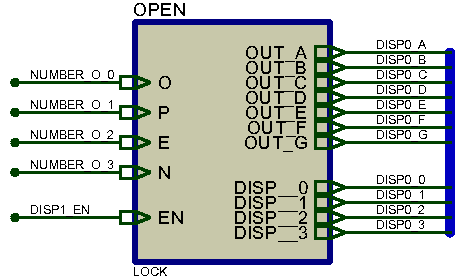
\includegraphics[scale = 1]{Graphics/OPEN-ERROR/OPEN-PARENT.PDF}
    \caption{Custom Fixed Open Message Driver}
    \label{fig:OPEN_DRIVER_PARENT}
\end{figure}

\begin{figure}[H]
    \centering
    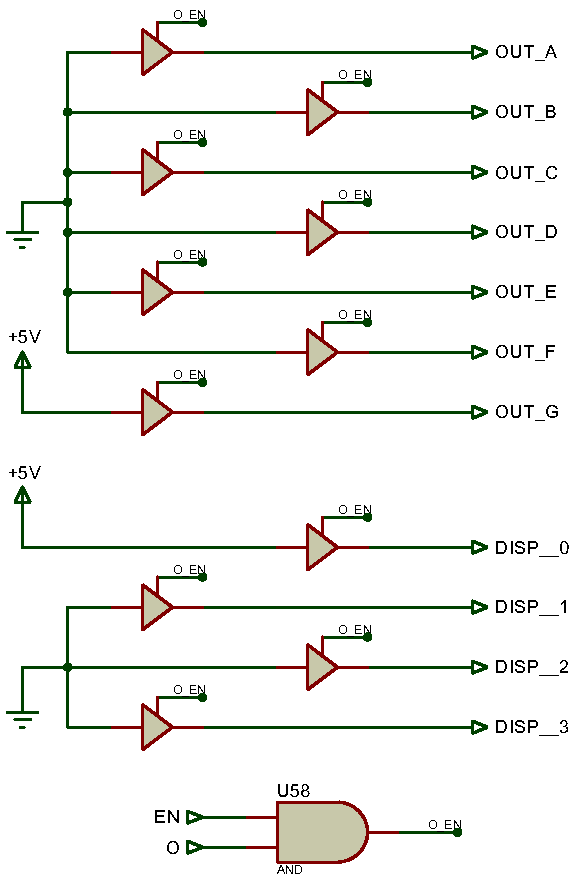
\includegraphics[scale = 0.8]{Graphics/OPEN-ERROR/OPEN-CHILD.PDF}
    \caption{Driver internals (Letter "O")}
    \label{fig:OPEN_DRIVER_CHILD}
\end{figure}

\medskip

These drivers take the \textit{NUMBER} signal as well as the ENABLE SELECTOR's \textit{ENABLE} one as inputs. When the GALs starts the ring, the \textit{ENABLE} signal is pulled HIGH, and based on the choice of the \textit{ENABLE SELECTOR} GAL (See \textbf{Subsection \ref{sec:ENABLE_AUTOSTART}} for more on this topic) the driver outputs both the display address, i.e., which 7-segment display needs to be turned on, as well as the state of the 7 segments. This allows us to create custom messages using a reduced amount of pins.\medskip

Of course, this method is rudimentary and not very efficient nor cost effective, but it was necessary for the correct visualization of the data.\medskip

To conclude, each time that the ring passes through \bm{$Q_4$}, i.e., the state corresponding to letter \textit{N}, the system checks the level of the \textit{RESET} signal. If it is in a HIGH level, the ring finishes and returns to state \textit{$Q_0$}. If it is on a LOW level, the loop continues. This effectively resets the GAL once the message displaying procedure is finished.\medskip

To illustrate the different states and the transitions between them we have included the following diagram:\medskip

\begin{figure}[H]
    \centering
    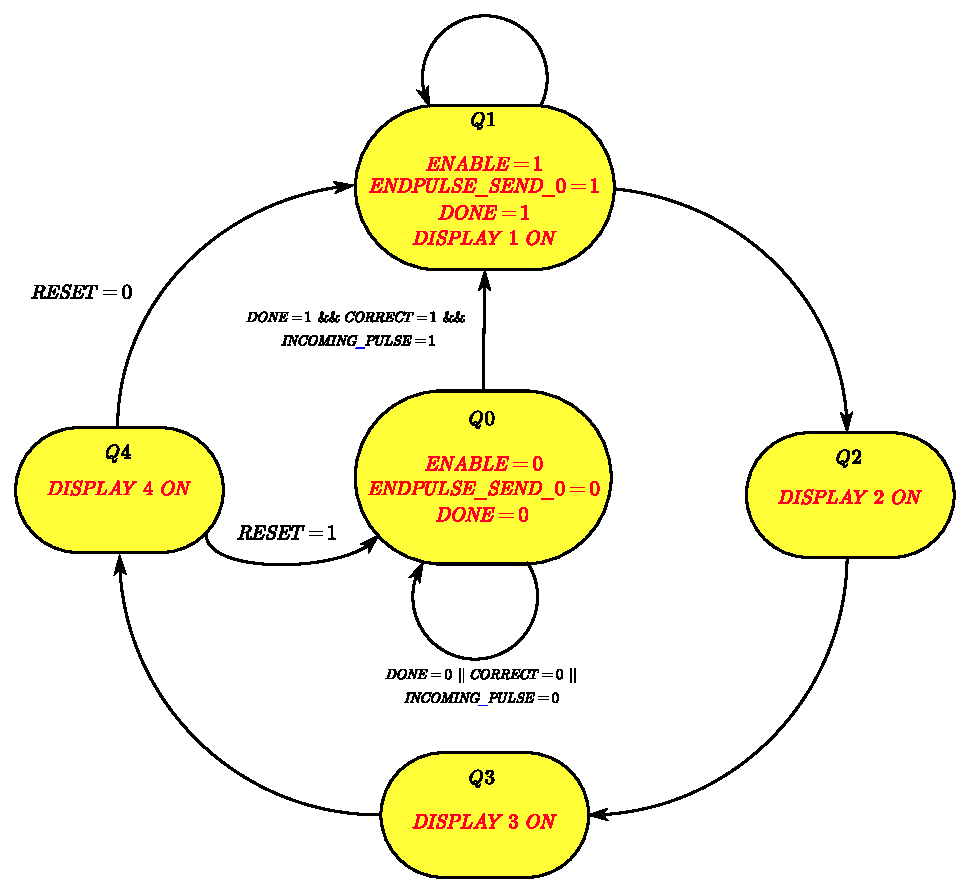
\includegraphics[scale = 0.75]{Graphics/OPEN-ERROR/OPEN_FSM.pdf}
    \caption{Open FSM}
    \label{fig:OPEN_FSM}
\end{figure}

\clearpage

The VHDL code that describes the process can be seen below:

\inputcode{Code/OPEN.vhd}

\clearpage

\subsubsection{\textit{Error} Message}
\medskip

The \textbf{\textit{Error}} message works in the same way as the \textbf{\textit{Open}} message, though there are two main differences:\medskip

\begin{itemize}
    \item The \textit{CORRECT} signal must be in a LOW level as we have to display the error message when the password entered by the user is incorrect.
    \item As the \textbf{\textit{Err}} message has three characters and not four, the fourth display and therefore the last state \textit{$Q_4$} are not used.
\end{itemize} \medskip

To illustrate the different states and the transitions between them we have included the following diagram:\medskip

\begin{figure}[H]
    \centering
    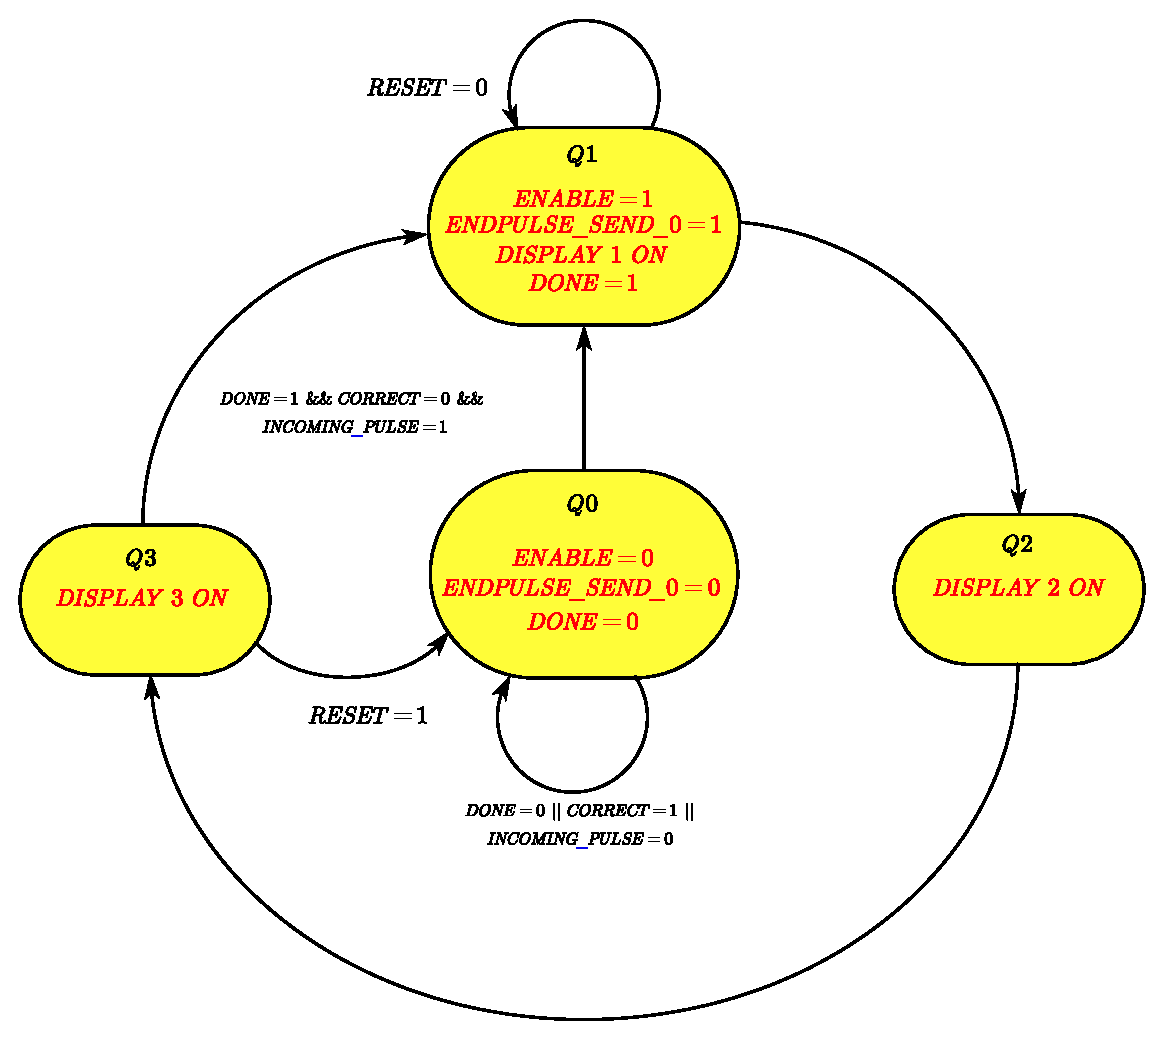
\includegraphics[scale = 0.6]{Graphics/OPEN-ERROR/ERROR_FSM.pdf}
    \caption{Error FSM}
    \label{fig:ERROR_FSM}
\end{figure}

\clearpage

The VHDL code that describes the process can be seen below:

\inputcode{Code/ERROR.vhd}

The Proteus Subassembly of both circuits is attached below:

\begin{figure}[H]
    \centering
    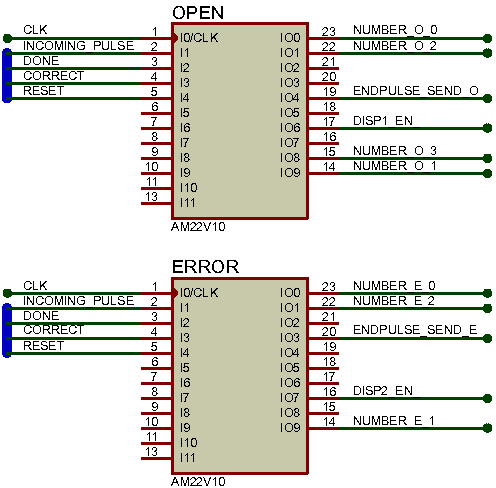
\includegraphics[scale = 1]{Graphics/OPEN-ERROR/OPEN_ERROR_PROTEUS.PDF}
    \caption{Open/Error Proteus Subassembly}
    \label{fig:OPEN_ERROR_PROTEUS}
\end{figure}

The custom driver for the \textbf{\textit{Err}} message, as well as its internals will not be shown as they are very similar to the one shown above.

\clearpage

\subsubsection{Final Roundup}

As per the last complex functional block, we will try to briefly go over the operation of the digit validation procedure since we know that it is a bit too hard to grasp. The different time-sensitive actions will be explained step by step.

\begin{enumerate}
    \item The code is introduced by the user
    
    \item Once the procedure described in \textbf{Subsubsection \ref{sec:STATE_FSM_DISPLAY_ROUNDUP}} is over (Storing the code in the RAM and displaying the introduced number), the \textit{DONE} signal is pulled HIGH.
    
    \item This signal is delayed approximately 0.5s to wait for the individual validation of the digits to occur (See \textbf{Subsection \ref{sec:IND_CHECK}} for more on this topic). 
    
    \item The delayed version of the \textit{DONE} signal arrives to the \textit{Password Checking} GAL, as well as the results of the individual digit checking procedure. If the introduced combination is correct, this GAL pulls \textit{CORRECT} HIGH, otherwise, it pulls it LOW. In either case, the GAL also pulls \textit{SENT\_PULSE} HIGH, which starts a 1 second delay in which the introduced digits are displayed.
    
    \item After 1 second, the delayed signal reaches the OPEN/ERROR GALs. Based on the state of the \textit{CORRECT} pin they decide whether to display the \textbf{\textit{Open}} message or the \textbf{\textit{Err}} one by pulling the corresponding \textit{ENABLE} pin HIGH. This pin is read by the ENABLE SELECTOR GAL, that is there to avoid short-circuiting the displays (See \textbf{Subsection \ref{sec:ENABLE_AUTOSTART}} for more on this topic). This last GAL turns on the correct driver, and the custom 7-segment display driver shows the appropriate message. At the same time, the \textit{ENDPULSE\_SEND} signal is pulled HIGH, activating yet another 1 second delay during which the \textit{Open}/\textit{Err} message is shown in the 4 7-segment displays. 
    
    \item After the 1 second delay is finished, the \textbf{\textit{RESET}} signal is pulsed and the whole systems restarts, allowing the user to introduce another password (See \textbf{Subsection \ref{sec:GENERAL_RESET}} for more on this).
\end{enumerate}



